\documentclass{beamer}
%%%%%%%%%%%%%%%%%%%%%%
% basic tutorial in german: http://www2.informatik.hu-berlin.de/~mischulz/beamer.html
%%%%%%%%%%%%%%%%%%%%%%

%------- packages ---------%
\usepackage[english]{babel}         %Umlaute, neue deutsche Rechtschreibung
\usepackage[utf8x]{inputenc}        %Kodierung festlegen, für UTF-8 Unterstützung entsprechend 
\usepackage{amsmath,amsfonts,amssymb}   %math. Symbole und Umgebungen
\usepackage{graphicx}
%\usepackage{natbib}
%\usepackage{animate} %need the animate.sty file 
\usepackage{color}

%------- theme and style ---------%
\usetheme{Boadilla}  %% Themenwahl
\usecolortheme{default}
\usefonttheme{default}
\useinnertheme{circles}     %	{circles | default | inmargin |	rectangles | rounded}
\useoutertheme{default} %	default | infolines | miniframes | shadow | sidebar | smoothbars |smoothtree | split | tree}
%\beamertemplatenavigationsymbolsempty   % disable navigation simbols
%\bibliographystyle{apalike}
%------- metainformation ---------%

\title[Bifurcation]{Bifurcation in parameter dependent systems\\~\\}
\subtitle{Numerical Methods for Systems Biology WS 12/13}
\author[Jonas Ibn-Salem]{Jonas Ibn-Salem}
\institute[]{}
\date{10.01.13}
%\logo{\pgfimage[width=2cm,height=0.5cm]{grafik/FULogo_RGB}}
\titlegraphic{
\includegraphics[width=4cm,height=1cm]{grafik/FULogo_RGB}}


\begin{document}
%\frame{\titlepage}
\maketitle


\begin{frame}{Overview}
    \tableofcontents
\end{frame}

%%%%%%%%%%%%%%%%%%%%%%%%%%%%%%%%%%%%%%%%%%%%%%%%%%%%%%%%%%%%%%%%%%%%%%%% 
\section{Introduction: Fixed Point Analysis}
%%%%%%%%%%%%%%%%%%%%%%%%%%%%%%%%%%%%%%%%%%%%%%%%%%%%%%%%%%%%%%%%%%%%%%%% 
\begin{frame}{Introduction: Fixed Point Analysis}
    Given the system of differential equations:
    $$y' = f(y) $$
    \begin{definition}
        A \emph{fixed point $y^*$} is defined by $f(y^*)=0$.
    \end{definition}
    %$\Rightarrow$ 
    \begin{itemize}
        \item Solve the equation $f(y) = 0$ 
        \item Analyse eigenvalues of the Jacobian at fixed points.
    \end{itemize}
\end{frame}
%%%%%%%%%%%%%%%%%%%%%%%%%%%%%%%%%%%%%%%%%%%%%%%%%%%%%%%%%%%%%%%%%%%%%%%% 
\section{Bifurcation}
%%%%%%%%%%%%%%%%%%%%%%%%%%%%%%%%%%%%%%%%%%%%%%%%%%%%%%%%%%%%%%%%%%%%%%%% 

\begin{frame}{Bifurcation}
    Now: System with \textcolor{blue}{\emph{controle parameter} $\mu$}. 
    $$y' = f(y, \textcolor{blue}{\mu})$${}    

    \begin{block}{}
    %    How does $\mu$ influence the number, location and stability of fixed points?
        How does $\textcolor{blue}{\mu}$ influence the fixed points?
    \end{block}

    \pause
    \begin{itemize}
        \item Change in FP stability
        \item Change in FP number and location.
    \end{itemize}
    
    \pause
    \begin{definition}
        \emph{Bifurcation} is the changing of the character of an equalibrium point and/or the creation of extra ones by alteration of a control parameter.
    \end{definition}

    The value of \textcolor{blue}{$\mu$} where bifurcation occurs is called a \emph{bifurcation point}.
\end{frame}

\subsection{Example: Logistig growth with harvesting}
\begin{frame}{Example: Logistig growth with harvesting}
    Growth of a (fish) population under harvesting (fishing):
    $$y' = \frac{1}{10}y(10 - y) - \textcolor{blue}{\mu} $$
%    $$y' = \frac{1}{10}y(10 - y) - \mu $$

    Solving $f(y,\mu) = 0$ for any parameter $\mu$. 
    %E.g. for $\mu = 0$ fixed points at $y=0$ and $y=10$.
    %For any parameter $\mu$: $\frac{1}{10}y(10 - y) - \mu = 0$
     \pause
     \begin{columns}
        \column{.3\textwidth}
            Fixed points at $y_{1/2} = 5 \pm \sqrt{25 - 10 \mu}$
            
            ~\\
            
            Stability: $\lambda = \frac{df}{dy} = -\frac{2}{10} y + 1$
        \column{.7\textwidth}
            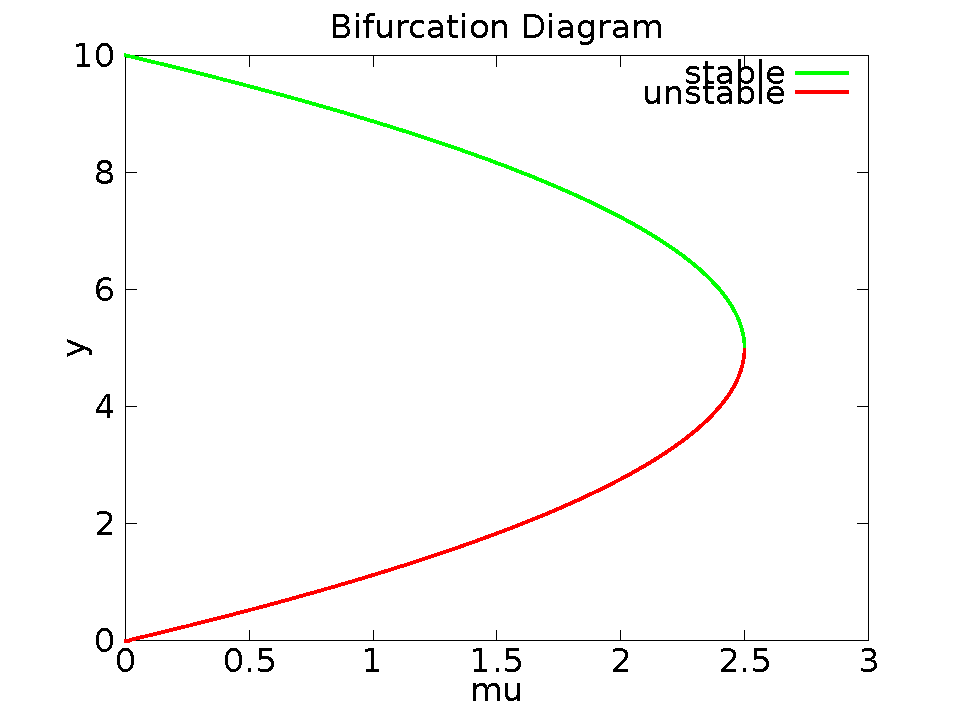
\includegraphics[width=1\textwidth]{grafik/harvesting}
    \end{columns}
\end{frame}

%%%%%%%%%%%%%%%%%%%%%%%%%%%%%%%%%%%%%%%%%%%%%%%%%%%%%%%%%%%%%%%%%%%%%%%% 
\section{Hopf Bifurcation}
%%%%%%%%%%%%%%%%%%%%%%%%%%%%%%%%%%%%%%%%%%%%%%%%%%%%%%%%%%%%%%%%%%%%%%%% 
\begin{frame}{Hopf Bifurcation}
    \begin{definition}
        A \emph{Hopf Bifurcation} is the appearance or disappearance of a periodic orbit (limit cycle) 
        through a local change in the stability properties of a fixed point.
    \end{definition}
    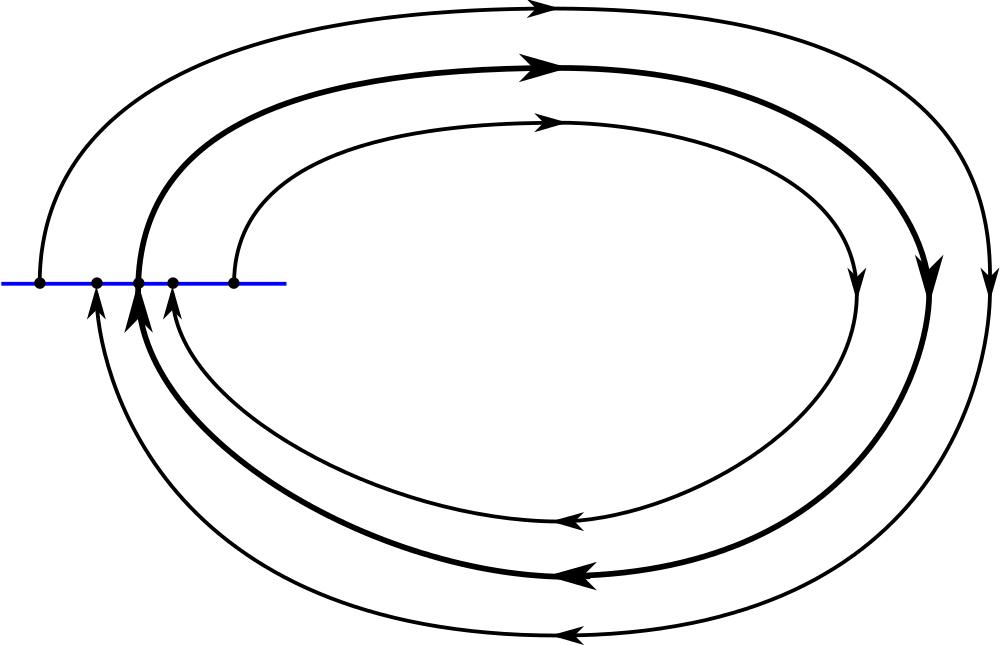
\includegraphics[width=.4\textwidth]{grafik/limitcycle}
    
    ~\\
    
    Appears when a pair of complex conjugate eigenvalues around the fixed point 
    crosses the imaginary axis of the complex plane.

        %\begin{align}
        %y_{1}' &= \mu - y_{1} - \frac{4 y_{1} y_{2} }{ y_{1}^{2} + 1} \\
        %y_{2}' &= y_{1} (1 - \frac{y_{2}}{y_{1}^{2} + 1})
        %\end{align}
        %\begin{align}
        %x' = - x + ay + x^2 y \\
        %y' = b - ay - x^2 y
        %\end{align}
\end{frame} 

\begin{frame}{Hopf Bifurcation example}
%    \begin{columns}
%        \column{.6\textwidth}
            \begin{exampleblock}{chlorine dioxide-iodine-malonic acid reaction}
                \begin{tabular}{l l}
                iodine: & $y_{1}' = \mu - y_{1} - \frac{4 y_{1} y_{2} }{ y_{1}^{2} + 1}$  \\
                chlorine dioxine: & $ y_{2}' = y_{1} (1 - \frac{y_{2}}{y_{1}^{2} + 1})$
                \end{tabular}
            \end{exampleblock}
%        \column{.4\textwidth}
            \begin{itemize}
                \item Fixed points at $(y_1, y_2) = (\frac{\mu}{5}, \frac{1}{25}(\mu^2 + 25) )$
                \item Bifurcation point at $\mu \approx 7.3$
            \end{itemize}
%    \end{columns}
     \begin{columns}
         \column{.5\textwidth}
         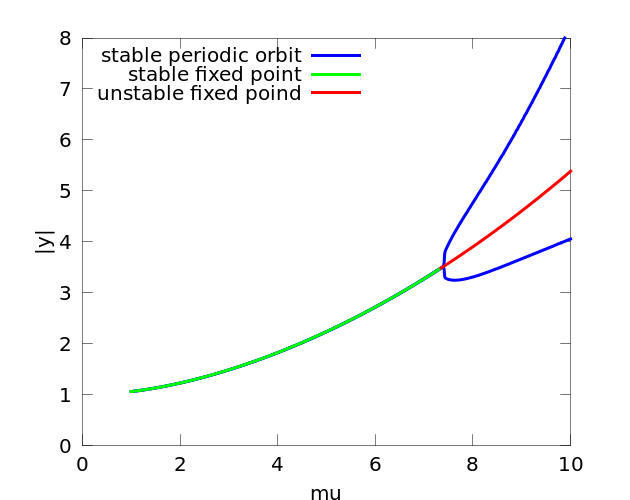
\includegraphics[width=\textwidth]{grafik/myrhshopf}
         %\animategraphics[autoplay,loop,height=5cm]{5}{grafik/Hopf-bif_}{0}{32} 
         \column{.5\textwidth}
         bla
     \end{columns}
\end{frame}

%%%%%%%%%%%%%%%%%%%%%%%%%%%%%%%%%%%%%%%%%%%%%%%%%%%%%%%%%%%%%%%%%%%%%%%% 
\section{Numerical Bifurcation Analysis: Path following}
%%%%%%%%%%%%%%%%%%%%%%%%%%%%%%%%%%%%%%%%%%%%%%%%%%%%%%%%%%%%%%%%%%%%%%%% 
\begin{frame}{Numerical Bifurcation Analysis}
    \begin{columns}
        \column{.6\textwidth}
        \begin{block}{}
            How to draw the bifurcation diagram and find bifurcation points?
        \end{block}
        \begin{itemize}
            \item Fixed point analysis for equidistant parameters $\mu$ is inefficient.
        \end{itemize}
        \column{.4\textwidth}
        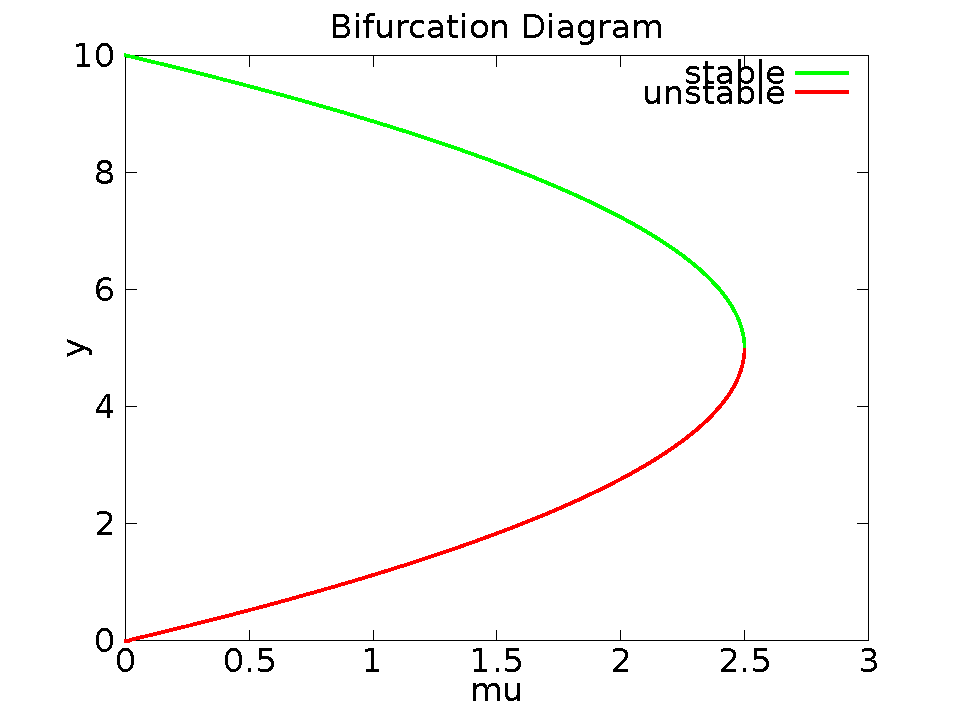
\includegraphics[width=\textwidth]{grafik/harvesting}
    \end{columns}
    
    \pause
    \begin{block}{Idea}
        Follow the fixed point around the fold bifurcation curve.
    \end{block}
    
    Treat $\mu$ as an aditional dependent variable in phase space and solve 
    $$f(y, \mu) = 0$$. 
    
\end{frame}

\begin{frame}{Numerical Bifurcation Analysis}
    
    \begin{itemize}
        \item Given two nearby points $z_{1} = (y_{1}, \mu_{1})$ and $z_2 = (y_2, \mu_2)$
        \item Initial approximation $ z_{a} = 2 z_{2} - z_{1}$
        \item Additional equation: $(z_3 - z_a) \cdot (z_a - z_2) = 0$
        \item Solving for $z_3$ via Newton's method with init. approx. $z_a$
    \end{itemize}
    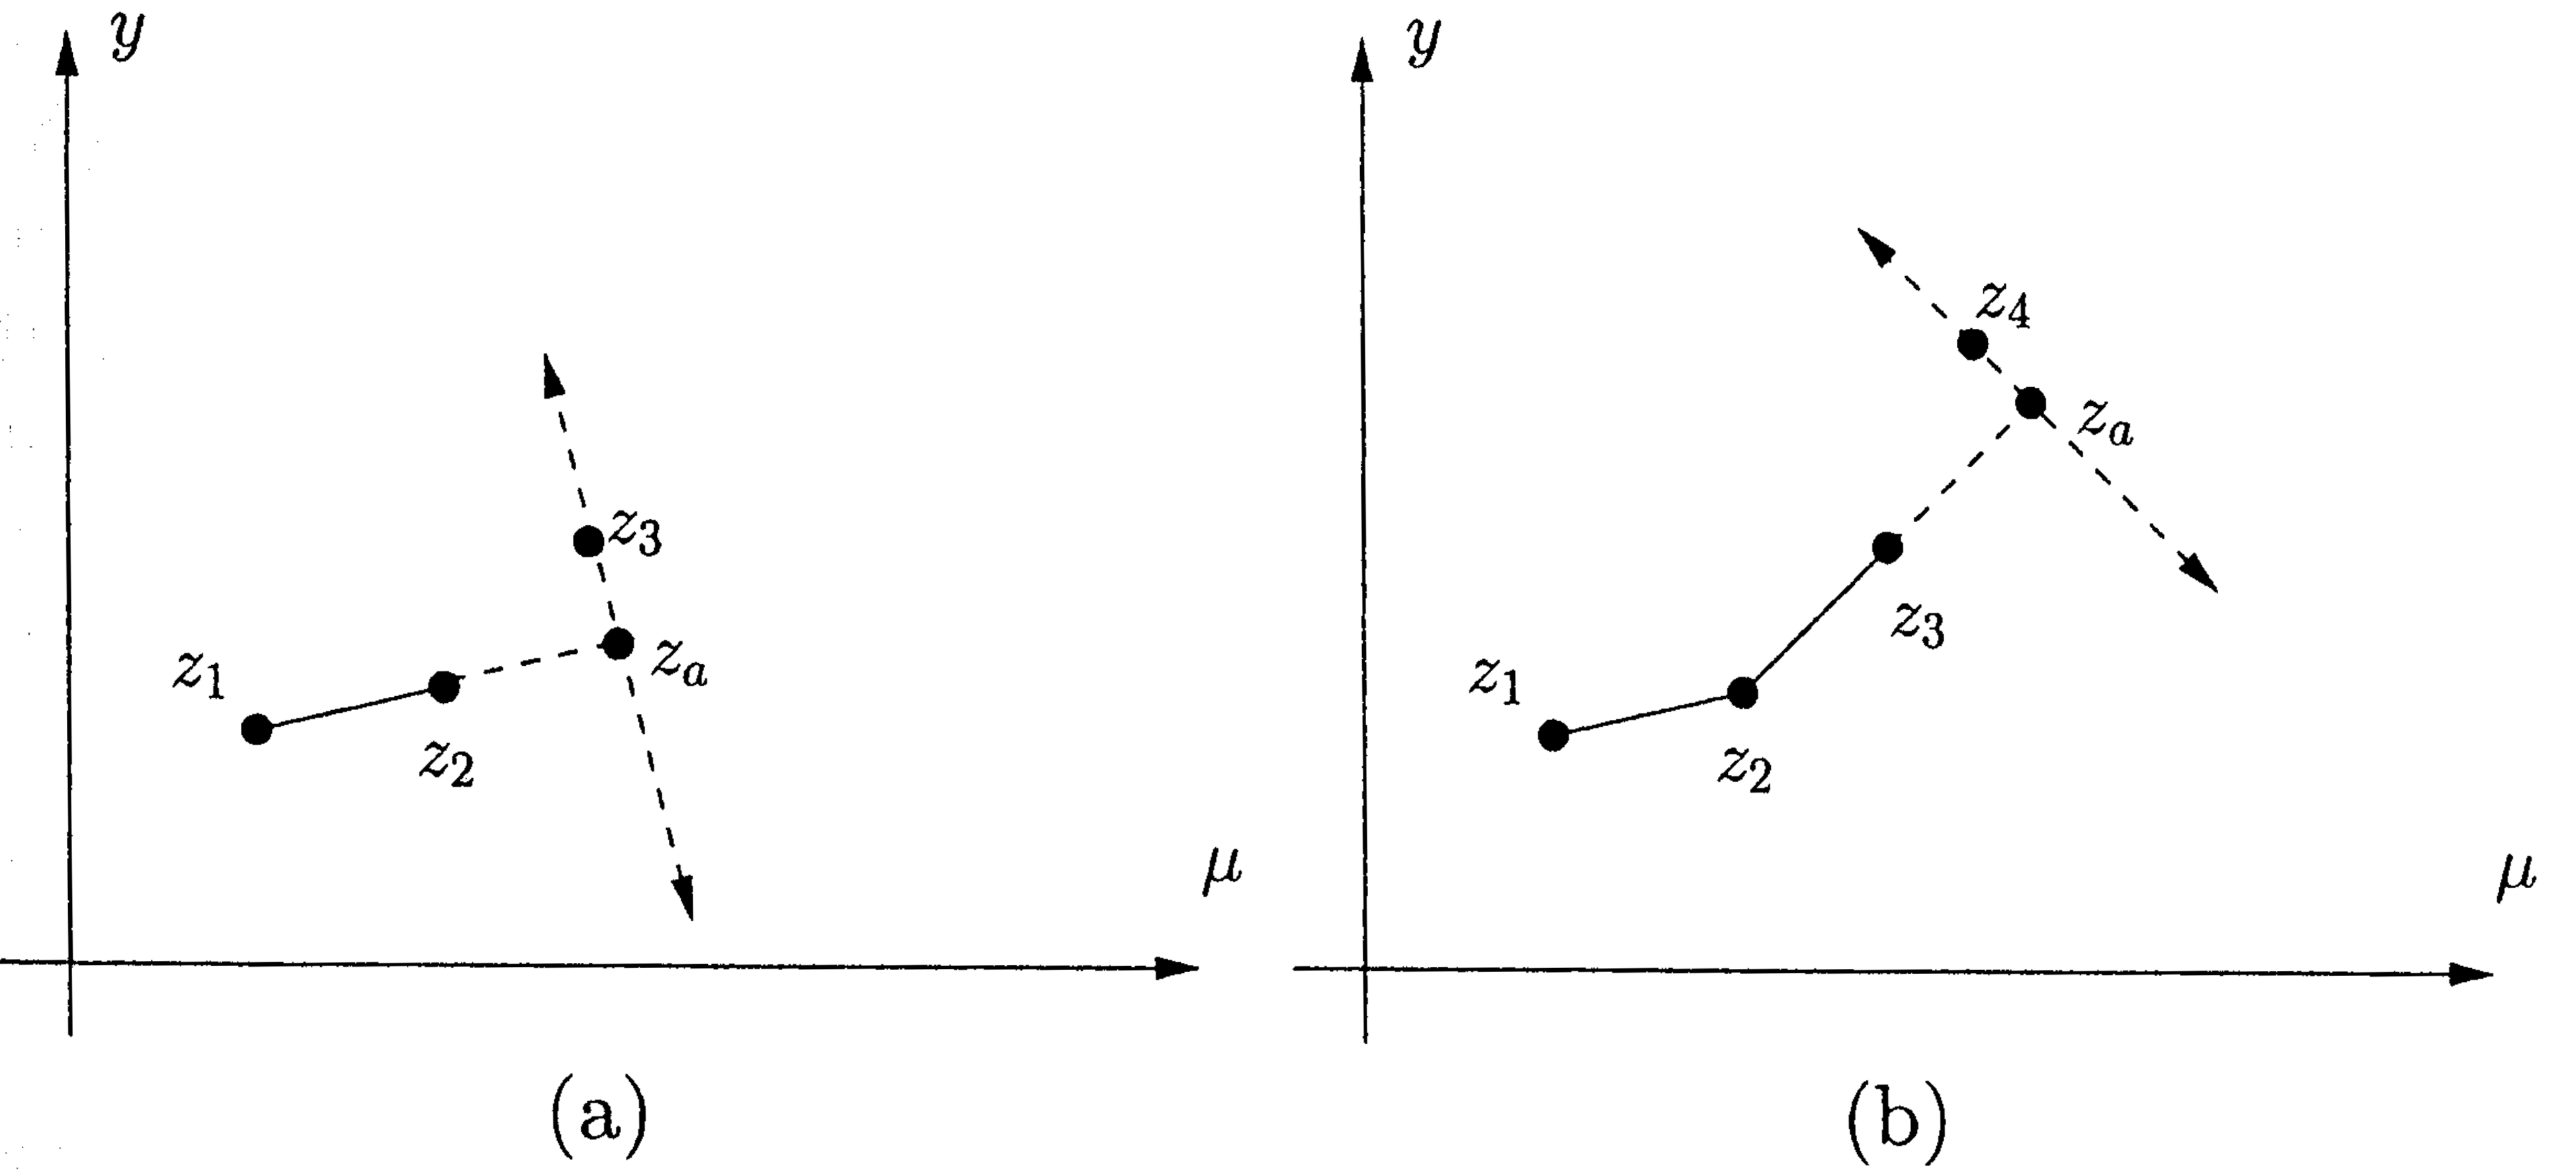
\includegraphics[width=\textwidth]{grafik/pathfollow}

\end{frame}

%\subsection{Path following}
%%%%%%%%%%%%%%%%%%%%%%%%%%%%%%%%%%%%%%%%%%%%%%%%%%%%%%%%%%%%%%%%%%%%%%%%
\begin{frame}{Example: Path following}
    Bifurcation Diagram for ~~ $y' = \mu y - y^3 $
    \begin{columns}
        \column{.5\textwidth}
        \begin{itemize}
            \item Fixing \textcolor{blue}{$\mu = -1$} yield $z_{1} = (0, -1)$ and $z_{2} = (0, -1 + \delta \mu)${}
            for small approximate distance $\delta\mu$
            \\
            %\begin{align}
            %     & \mu_{1} = -1                & \Rightarrow ~ z_{1} = (0, -1)  \\
            %     & \mu_{2} = -1 + \delta \mu  &\Rightarrow ~ z_{2} = (0, -1 + \delta \mu)
            %\end{align}
        \end{itemize}
        \pause
        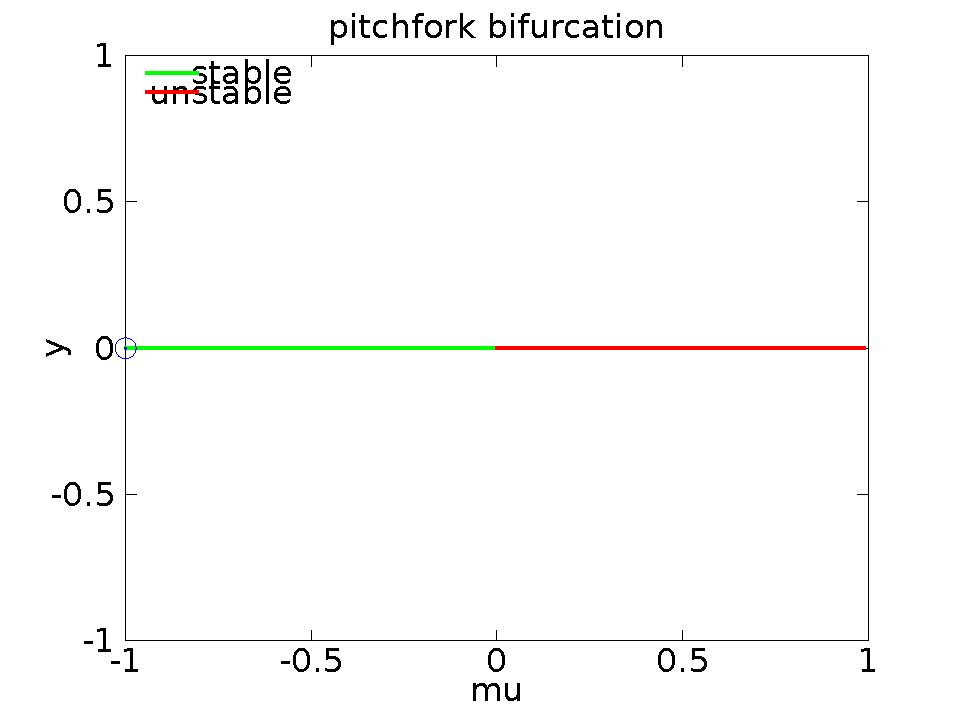
\includegraphics[width=1\textwidth]{grafik/pfexample1}
        \pause
        \column{.5\textwidth}   
        \begin{itemize}
            \item Other fixed points for \textcolor{blue}{$\mu = 1$} yield $z_{1} = (1, 1)$ and $z_{2} = (1, 1 - \delta \mu)$
            %\item $\lambda = \frac{df}{dy} = \mu - 3*y^2$
            \\
            %\begin{align}
            %     & \mu_{1} = -1                & \Rightarrow ~ z_{1} = (0, -1)  \\
            %     & \mu_{2} = -1 + \delta \mu  &\Rightarrow ~ z_{2} = (0, -1 + \delta \mu)
            %\end{align}
        \end{itemize}
        ~\\
        ~\\
        
        \pause
        
        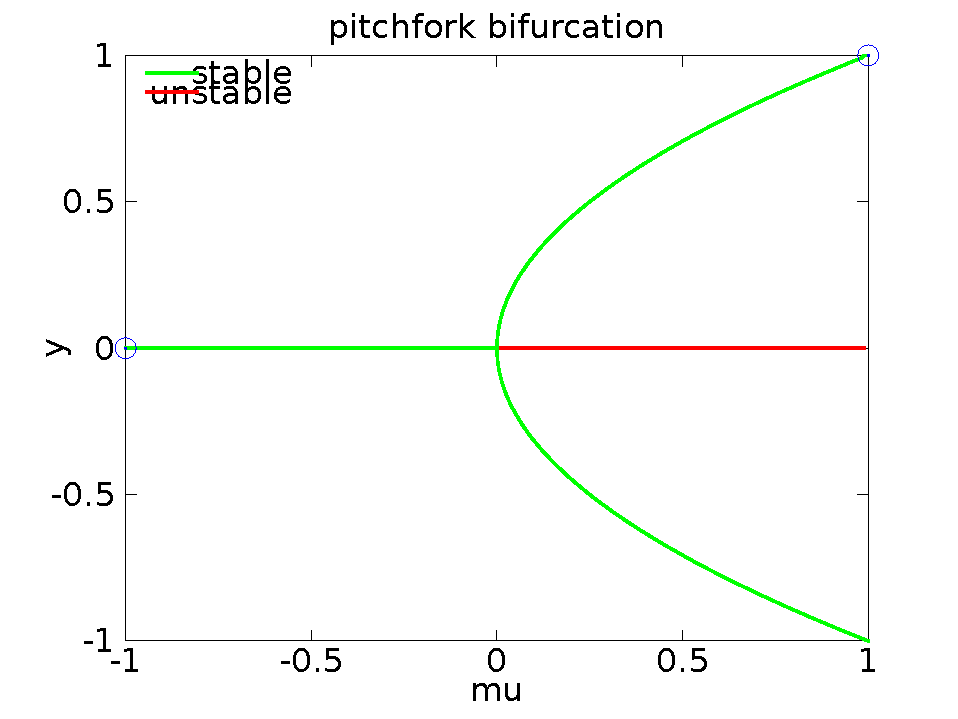
\includegraphics[width=1\textwidth]{grafik/pfexample2}
        
    \end{columns}
\end{frame}

\begin{frame}{Summary}
    \begin{itemize}
        \item Controle parameters can influce fixed points in ODE systems.
        \item At bifurcation points, the stability, location and/or number of fixed points change. 
        \item In a Hopf bifurcation a fixed point loses stability and a limit cycle occours.
        \item Bifurcation can be analysed numerically using path following.
    \end{itemize}

~\\
~\\
    \small
    Sources:
    \begin{itemize}
        \small \item D.S. Jones et al.: \emph{Differential Equations and Mathematical Biology.} CRC Press (2010)
    \end{itemize}

\end{frame}


%\usebackgroundtemplate{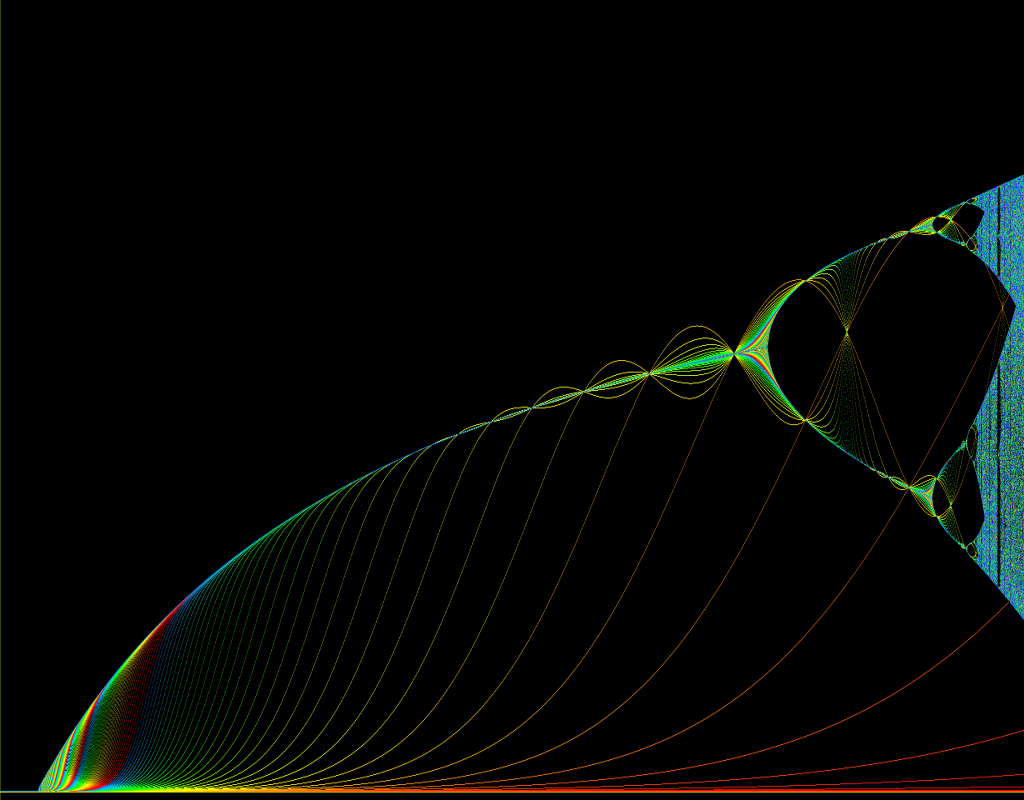
\includegraphics[height=\paperheight]{grafik/chaos}} 
\beamertemplatenavigationsymbolsempty
\usebackgroundtemplate{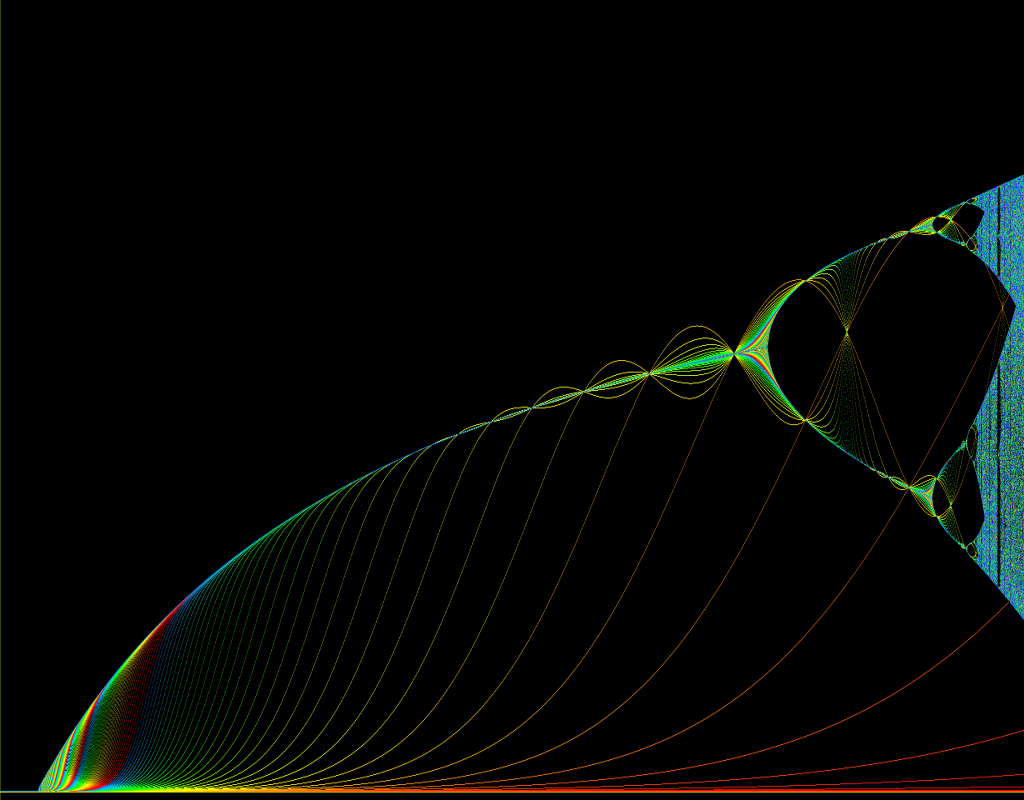
\includegraphics[width=\paperwidth]{grafik/chaos}} 
\begin{frame}{Thank you!}
    
\end{frame}

\end{document}

\begin{comment}
Gif animation with adope presentation:
http://www.ipgp.fr/~lucas/Contrib/animbeamer.html
\end{comment}
